\documentclass{article}%
\usepackage[T1]{fontenc}%
\usepackage[utf8]{inputenc}%
\usepackage{lmodern}%
\usepackage{textcomp}%
\usepackage{lastpage}%
\usepackage{authblk}%
\usepackage{graphicx}%
%
\title{The costimulatory immunogen LPS induces the B{-}Cell clones that infiltrate transplanted human kidneys}%
\author{Bonnie Edwards}%
\affil{Center for Microbial Interface Biology, Department of Microbial Infection and Immunity, The Ohio State University, Columbus, Ohio, United States of America}%
\date{01{-}01{-}2013}%
%
\begin{document}%
\normalsize%
\maketitle%
\section{Abstract}%
\label{sec:Abstract}%
SAN DIEGO (KGTV) {-} After years of study, a San Diego scientist discovered a protein hidden in human urothelial bladder tumors that may offer another way to find a way to fight prostate cancer.\newline%
What if that prostate cancer turned out to be something most men would like to be aware of?\newline%
In a study conducted at UC San Diego's Center for Biomedical Analysis, Jirik Ladia analyzed low{-}grade bladder cancer tumors, using a new method called extracellular microscopy.\newline%
RELATED: 'Secretly' back in clinical trials\newline%
In this highly specific way, MRI or X{-}ray scanning techniques beam a single photo to the multiple tumors and then separates them into small groups according to which cancers the larger images identify as breast, liver, kidney, lung, cardiovascular, eye, bladder and colon.\newline%
Results showed that fumaric acid (an alcohol molecule found in urine) was found to contain a high concentration of fumaric acid, the metabolite found in every cell of the bladder stem.\newline%
Even more surprising, Ladia found that chemokine was a more potent target for blocking the stem activity than previously thought, with a 45 percent relative rate when chemicals other than fumaric acid were blocked.\newline%
RELATED: Scholar unveils new UC San Diego lab\newline%
This finding is good news not only for cancer patients, but for patients who choose to avoid high levels of fumaric acid, Ladia said.\newline%
"I think it's great that if there is a man in the bar who can't come in right now, maybe these prostate cancer patients can look at this test and stick with their doc for a few weeks," Ladia said.\newline%
Baron Laboratories is the company that developed this new test for bladder cancer.

%
\subsection{Image Analysis}%
\label{subsec:ImageAnalysis}%


\begin{figure}[h!]%
\centering%
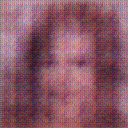
\includegraphics[width=150px]{500_fake_images/samples_5_392.png}%
\caption{A Black And White Photo Of A Black And White Cat}%
\end{figure}

%
\end{document}